%!TEX root = ../doc.tex
\chapter{Prototyp}
\label{sec:prototyp}


\section{Tools}
\subsection{Entwicklungsumgebung}
Für die Versionsverwaltung wird Github\footnote{\url{https://github.com/roosnic1/zhaw_bachelor}} verwendet. Als Entwicklungsumgebung wurde auf WebStorm\footnote{WebStorm Version: 2016.1.3} von JetBrians\footnote{\url{https://www.jetbrains.com/webstorm/}} zurückgegriffen. WebStorm bietet viele Tools für effizientes Programmieren in JavScript. Zum einen hilft WebStorm die Programmierstandards einzuhalten und vervollständigt viele Eingaben automatisch. Eine zusätzliche grosse Hilfe ist die Erkennung von \textit{NPM Tasks}, welche dann als eine ausführbare Konfiguration abgespeichert werden können. Dadurch lässt sich die gesamte Entwicklungsumgebung mit wenigen Handgriffen aus einem Programm starten.

\subsection{Browser}
Für das Ausführen der Single-Page Applikaiton wurde die neuste Version des Google Chrome Canary\footnote{Version: 54.0.2793.0 canary (64-bit)} Browsers verwendet. Zusätzlich wurden zwei Browser Erweiterungen installiert mit welchen die Entwicklung und das Testen verbessert wurde.

\subsubsection{React Erweiterung}
Die React Browser Erweiterung erlaubt es den Zustand einer React Komponente zur Laufzeit zu inspizieren. Die Übergebenen Parameter sowie die Verfügbaren Eigenschaften werden angezeigt und können auch angepasst werden. Der Inhalt des \textit{Stores} sowie der des Komponenten internen Status sind verfügbar. In Abbildung \ref{fig:reactext} ist die Ansicht der React Browser Erweiterung mit der OrdersStep2 Komponente zu sehen.

\begin{figure}[ht]
	\centering
  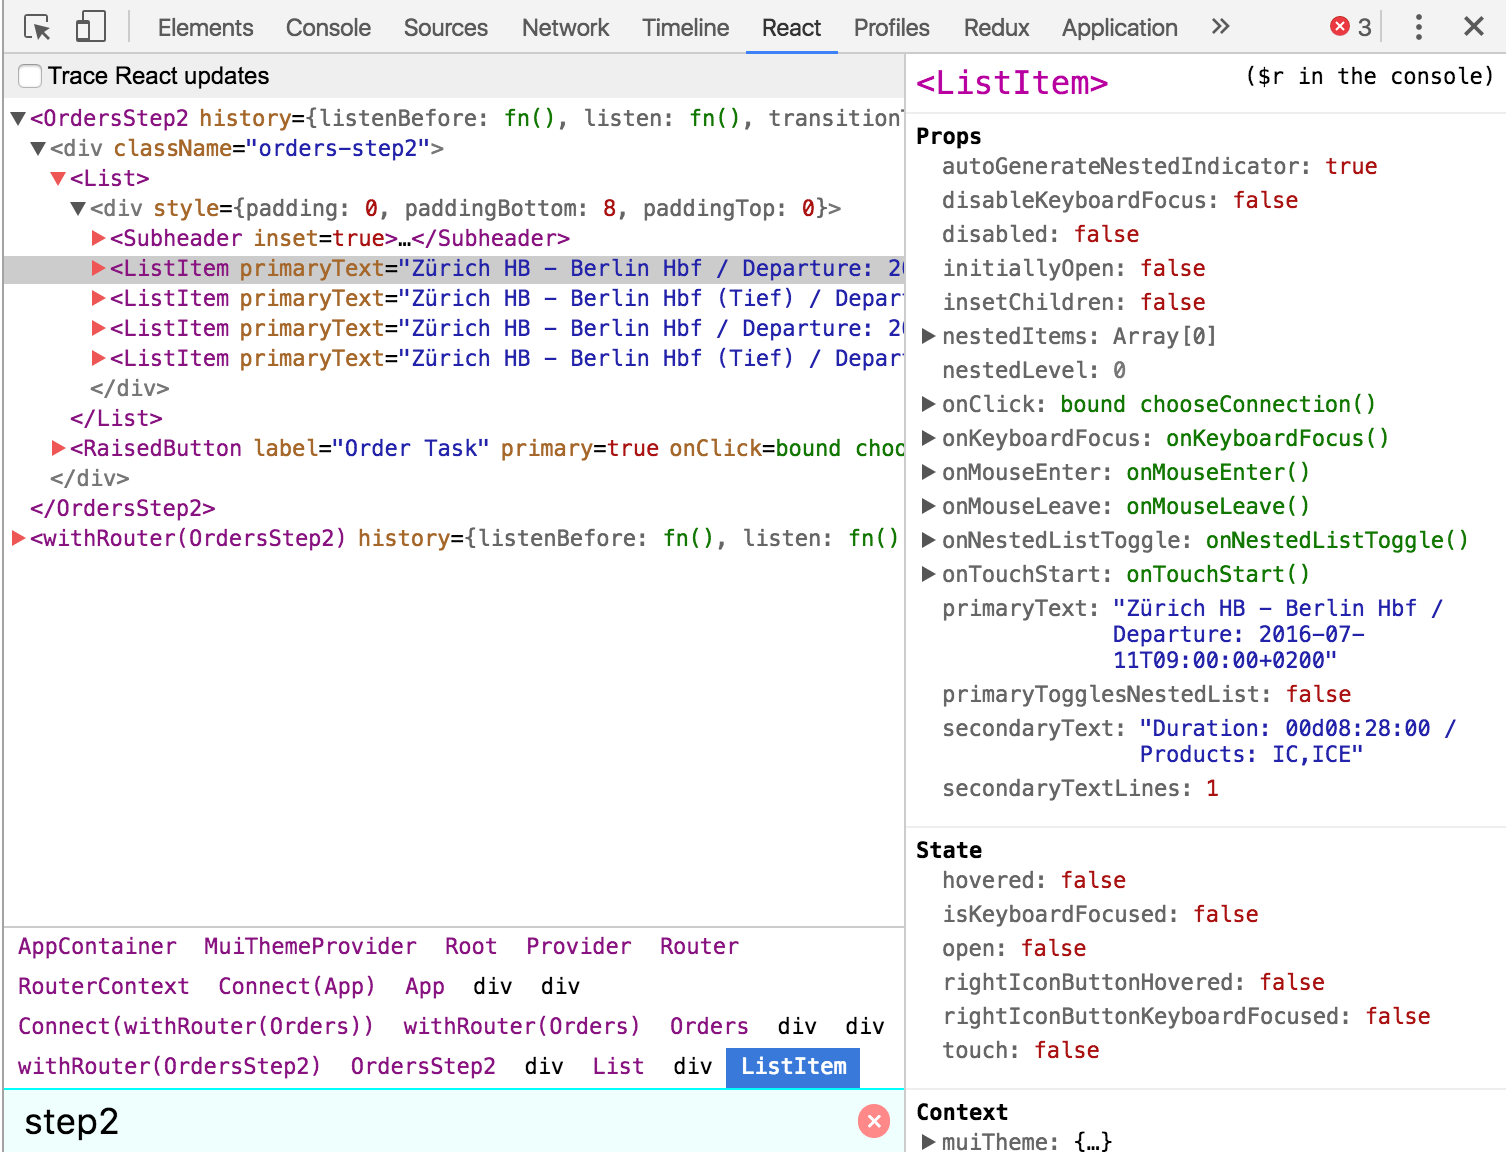
\includegraphics[width=0.88\textwidth]{images/reactext.png}
	\caption{React Browser Erweiterung}
	\label{fig:reactext}
\end{figure}

\subsubsection{Redux Erweiterung}
Die Redux Browser Erweiterung zeichnet alle ausgeführten Aktionen auf und listet diese auf einer Zeitachse auf. Die Aktionen können inspiziert und wieder rückgängig gemacht werden. Es wird aufgezeigt wie der Zustand des \textit{Stores} vor und nach der Aktion aussieht. In Abbildung \ref{fig:reduxext} ist die Ansicht der Redux Browser Erweiterung zu sehen.

\begin{figure}[H]
	\centering
  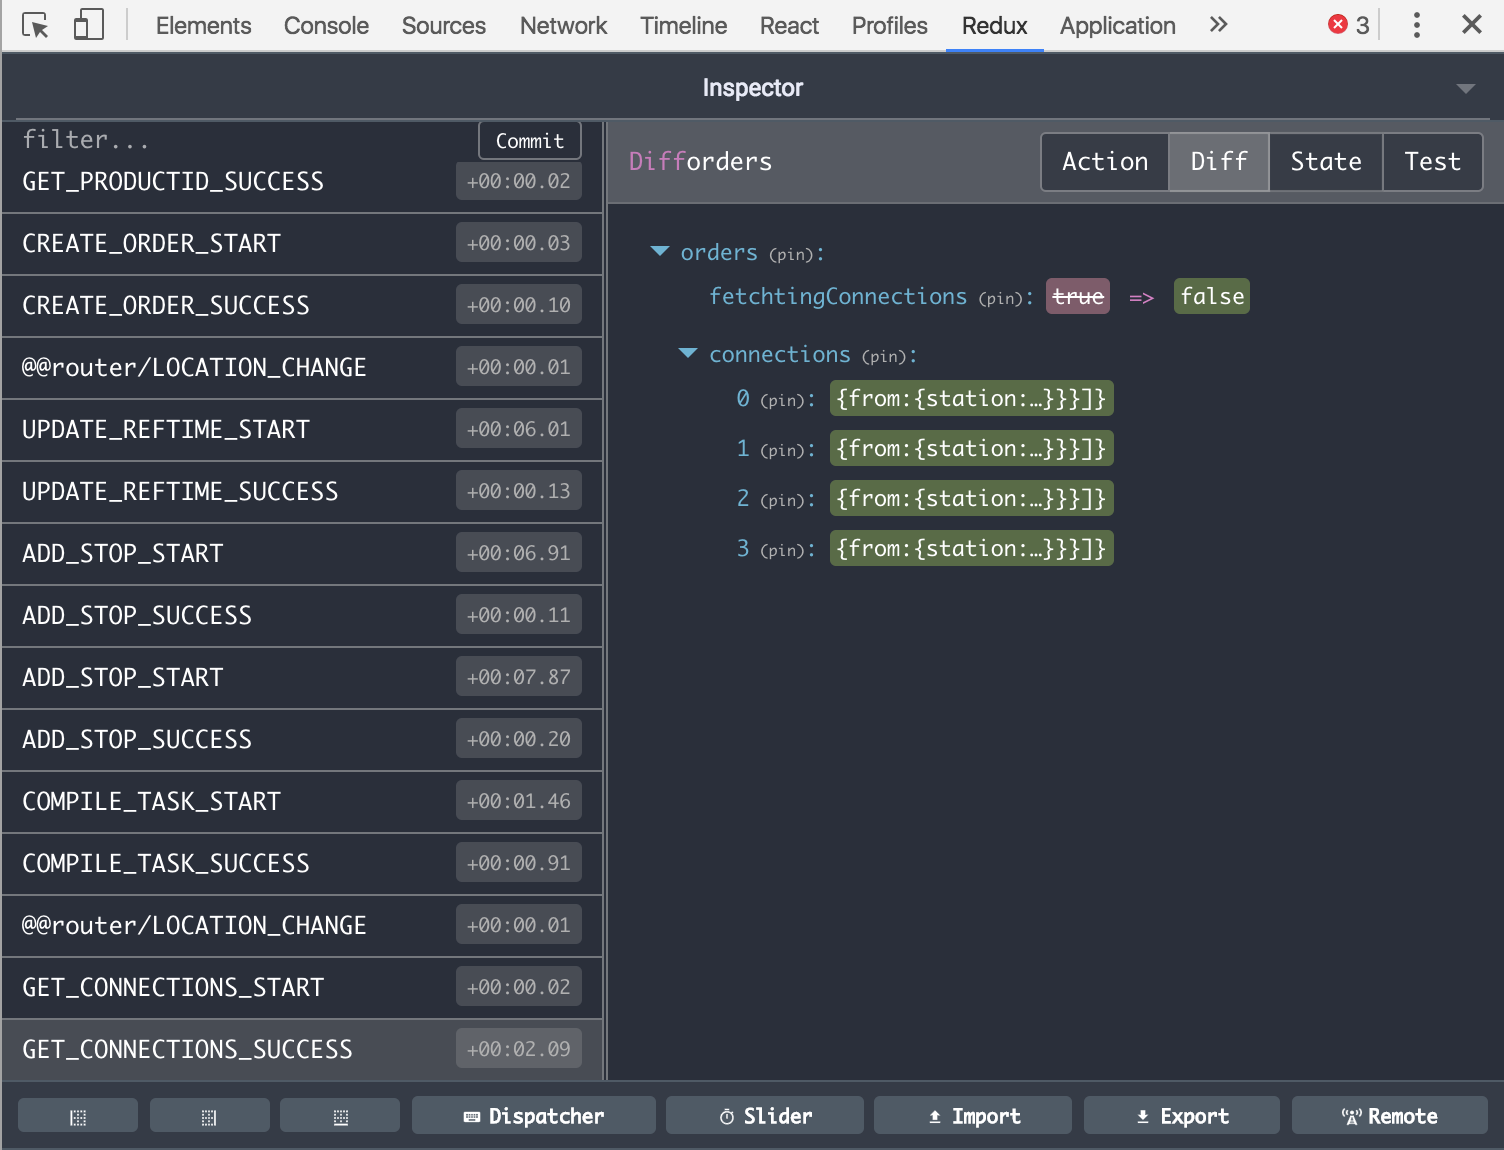
\includegraphics[width=0.88\textwidth]{images/reduxext.png}
	\caption{Redux Browser Erweiterung}
	\label{fig:reduxext}
\end{figure}


\subsection{Test Server}
Als Test Server wurde ein virtueller Ubuntu 16.04 Server verwendet. Als Webserver wurde nginx\footnote{\url{https://nginx.org}} verwendet. Der Webserver funktioniert als Proxy für den lokal laufende Node.js Webserver. Für Node.js wurde \textit{pm2}\footnote{\url{https://github.com/Unitech/pm2}} verwendet. Mit \textit{pm2} werden Node.js Prozesse überwacht, deren Standard Ausgabe abgefangen und gespeichert und im Falle eines Absturzes neu gestartet.

\section{Codebasis}
Für die Entwicklung wurde auf einer \textit{ToDo} Single-Page Applikation aufgebaut. Viele Software Frameworks oder Software Paradigmen werden in einem ToDo Projekt vorgestellt und lassen sich als Start für eigene Projekte verwenden. Im Rahmen dieser Bachelorarbeit wurde auf das \textit{ToDo-React-Redux} Projekt von Richard Park auf Github\footnote{\url{https://github.com/r-park/todo-react-redux}} zurückgegriffen. Das Projekt implementiert eine einfach ToDo Applikation mit React und Redux. Die Daten werden mit Firebase\footnote{Firebase ist ein \textit{Backend as a Service} Anbieter. \url{https://firebase.google.com/}} synchronisiert und benötigen deshalb eine asynchrone Handhabung. Dies ist hilfreich, weil die Kommunikation mit dem Mini-Backend auch asynchron stattfindet. Zusätzlich verwendet das Projekt Wekzeuge wie Webpack, Babel, React-Redux und ESLint welche im Folgenden genauer beschrieben werden.

\subsection{Webpack}
Webpack\footnote{\url{https://github.com/webpack/webpack}} ist ein modernes Werkzeug welches hilft eine grosse Codebasis in statische Dateien zu transformieren. Diese statischen Daten können dann zur Verwendung in einer Produktiven Umgebung verwendet werden. Die neuste Version von JavaScript erlaubt es einfach Inhalte zu exportieren beziehungsweise zu importieren. Dadurch kann die Applikation in viele verschiedene Teile aufgeteilt werden, welche am Anfang ihres Codeteils auf diejenigen Codeteil verweisen die zusätzlich benötigt werden. Diese Abhängigkeiten werden von Webpack für einen erfolgreichen produktiven Einsatz gelöst. Zusätzlich ermöglicht Webpack mit sehr wenigen Zeilen einen lokalen Webserver zu starten. Im Folgenden ist die Konfiguration für den verwendeten lokalen Webserver.
\begin{lstlisting}[caption=Lokaler Webserver]
  config.devServer = {
    contentBase: './src',
    historyApiFallback: true,
    host: HOST,
    hot: true,
    port: PORT,
    publicPath: config.output.publicPath,
    stats: {
      cached: true,
      cachedAssets: true,
      chunks: true,
      chunkModules: false,
      colors: true,
      hash: false,
      reasons: true,
      timings: true,
      version: false
    },
    proxy: {
      '/api/v1/*': {
        target: 'http://localhost:3001',
        secure: false
      }
    }
  };
\end{lstlisting}
Dieser lokale Webserver ist nur für die SPA zuständig und reagiert nur auf deren Dateiänderungen während der Entwicklung. Für das Mini-Backend wird ein eigener lokaler Webserver verwendet, welcher nur auf Dateiänderungen im Mini-Backend reagiert. In einer Produktiven Umgebung werden SPA sowie Mini-Backend vom gleichen Webserver bedient, was zum Problem führt dass während der Entwicklung die Anfragen an das Mini-Backend umgeleitet werden müssen. In Webpack ist dies mit dem Parameter Proxy möglich, welcher alle Anfragen auf eine gewisse URL umleitet.


\subsection{Babel}
Babel\footnote{\url{https://babeljs.io/}} ist ein JavaScript transpiler, welcher es erlaubt die neuste Version von JavaScript für alle Browser ausführbar zu machen. Obwohl die neuste Version von JavaScript bereits im Juni 2015 veröffentlicht wurde, sind noch nicht alle Browserhersteller in der Lage all diese Erneuerungen in ihren Browser auszuführen. Babel transpiliert diesen neuen Code in Bekannten JavaScript ES5 Code, welcher selbst von älteren Browsern ausgeführt werden kann. Babel wird mit Webpack verwendet und hat den grossen Vorteil, dass die Codebasis auf viele neue und bessere Programmiereigenschaften zugreifen kann.

\subsection{React-Redux}
React-Redux\footnote{\url{https://github.com/reactjs/react-redux}} ist eine Erweiterung für React und Redux welche die beiden Frameworks miteinander verbindet. Redux sieht vor dass es nur einen \textit{Store} gibt, welche alle Daten für die gesamte Applikation beinhaltet. Dieser Store wird auf der obersten Ebene von React definiert und einer Provider Komponente übergeben.

\begin{lstlisting}[caption=Root Komponente]
export default function Root({history, onEnter, store}) {
  return (
    <Provider store={store}>
      <Router history={history}>
        <Route component={App} onEnter={onEnter} path="/">
          <IndexRoute component={Home} />
          <Route component={Orders} path={ORDERS_PATH}>
            <IndexRoute component={OrdersStep1} />
            <Route component={OrdersStep2} path={ORDERS_PATH + '/step2'} />
            <Route component={OrdersStep3} path={ORDERS_PATH + '/step3'} />
            <Route component={OrdersStep4} path={ORDERS_PATH + '/step4'} />
          </Route>
          <Route component={SignIn} path={SIGN_IN_PATH} />
          <Route component={Tasks} path={TASKS_PATH} />
        </Route>
      </Router>
    </Provider>
  );
}
\end{lstlisting}

Damit dieser Store nicht durch alle Subkomponenten durchgereicht werden muss, wird mit react-redux das Werkzeug \textit{connect} zur Verfügung gestellt. Damit ist es möglich bei der Definition einer Komponente zu definieren welchen Teil des \textit{Stores} in der Komponente bereit gestellt werden soll. Im Folgenden Codebeispiel ist zu sehe wie ein Teil des \textit{Stores} der Orders Komponente mit \textit{connect} zur Verfügung gestellt wird.
\begin{lstlisting}[caption=connect im Einsatz]
export default connect(state => {
  return {
    orders: state.orders
  };
}, Object.assign({}, ordersActions))(Orders);
\end{lstlisting}

\subsection{ESLint}
ESLint\footnote{\url{http://eslint.org/}} ist ein JavaScript linter welcher auf Plugins aufbaut. Im Gegensatz zu anderen Codelintern ist ESLint in der Lage JSX Code zu interpretieren und macht ihn geeignet für React Softwareprojekte. Ein Linter trägt stark zur Qualität und Verwaltbarkeit von Softwareprojekten bei.

\section{Entwicklungsprozess}
\subsection{Mini-Backend}
API endpunkte entwickeln.
Lobo requests erstell methode.
Lobo limmitierung. keine polygone. Versorgungs gebiete selber erstellen. Polygon mit lat und lng erstellen. überprüfen ob punkt drin liegt.
%http://iso4app.net/ für die polygone
%https://github.com/tmpvar/polygon.js
%https://www.npmjs.com/package/vec2

???Error handling


\subsection{SPA}
aktion erstellen (XYZ_START, XYZ_SUCCESS, XYZ_ERROR)
reducer und State (pure functions ???)
Komponente erstellen



